\documentclass[a4paper,10pt]{article}

\usepackage[utf8]{inputenc}
%\usepackage[T1]{fontenc}

\usepackage{textcomp}           % Extra Symbole (Grad Celsius etc.)
\usepackage{amssymb,amsmath}    % Schöne Formeln (AMS = American Mathematical Society)
\usepackage{graphicx}           % Bilder und Seitenränder
\usepackage{subcaption}			% captions for subfigures
\usepackage{booktabs}           % Schönere Tabellen
\usepackage{colortbl}           % Farbige Tabellen

%\usepackage{tcolorbox}			% schöne bunte Boxen
\usepackage{mathtools}			% \mathclap für ordentliche \underbrace-			environments
\usepackage[left=2cm,right=2cm,top=2cm,bottom=2cm]{geometry}			% Pagelayout mit \newgeometry, \restoregeometry
\usepackage{float}
\usepackage{wrapfig}
\usepackage{enumitem}
\usepackage{float}
\usepackage{braket}
\usepackage{caption}
\usepackage[per-mode=fraction,output-decimal-marker={.},binary-units=true,separate-uncertainty=true]{siunitx}
\usepackage[breaklinks=true,colorlinks=true,linkcolor=blue,urlcolor=blue,citecolor=blue]{hyperref}
\usepackage{physics}
\usepackage{url}
\usepackage{subcaption}
\usepackage{calrsfs}
\DeclareMathAlphabet{\pazocal}{OMS}{zplm}{m}{n}
\usepackage{tikz}
\usetikzlibrary{decorations, positioning, intersections, calc, shapes,arrows, scopes}
\usepackage{pgfplots}
\usepackage{bodegraph}
\usepackage{circuitikz}
\usepackage{chemfig}
\usepackage{chemformula}
\graphicspath{{./img/}}
\usepackage{verbatim}

\DeclareSIUnit\elementarycharge{e}

\newcommand{\dif}{\mathrm{d}}

\bibliographystyle{unsrtnat}

\renewcommand{\k}{\mathbf{k}}
\begin{document}
\begin{titlepage}
 \begin{center}
	\Large{Advanced laboratory course 3}
	\end{center}
	\begin{center}
	 \LARGE{\textbf{FP3 - High Resolution Mass Spectroscopy}}
	\end{center}

	\begin{center}

	\large Marco \textsc{Canteri} \\
	marco.canteri@student.uibk.ac.at\\
	\large Maximilian \textsc{Münst} \\
	maximilian.muenst@student.uibk.ac.at
	\end{center}

	\begin{center}
	\vspace{1cm}
	Innsbruck, \today
	\vspace{1cm}
	\end{center}

	\begin{abstract}
		In the course of this experiment a high resolution long time measurement of the mass spectrum of Angiotensin was conducted using a FT-ICR mass spectrometer. Furthermore, fragments of CID collision were recorded over a collision energy range from \num{0} to \SI{20}{\electronvolt}. Finally, mass spectra of SORI-CID fragments were measured for several SORI-power settings. 
    \end{abstract}
    \vspace{1cm}

	\begin{center}
	
\includegraphics[scale=0.4]{img/uibk}
	\end{center}

\end{titlepage}


\section{Introduction}
In this experiment a Fourier-transform ion cyclotron mass spectrometer is used as a means to gather basic experiences on working with high resolution mass spectrometry. The ability to perform high resolution mass spectrometry is of key importance in many fields of research in physics and chemistry. Furthermore, there is a manifold of applications in chemical and pharmaceutical industries. 

\section{Theoretical Background}
\label{sec_theory}
In this section a concise overview is given over the ideas behind the way a Fourier-transform ion cyclotron resonance mass spectrometer works. The setup used is presented in the next section. 

\subsection{Ion Cyclotron Resonance Mass Spectroscopy}
The principal idea is that the mass-to-charge ratio of a charged ion can be determined by circulation of a group of ions in a magnetic field. This introduction is based on \cite{primer}. One can begin with the centripetal force necessary to maintain a circular movement, which is given by the Lorentz force
\begin{equation}
	\frac{m v^2}{r} = q v B,
\end{equation}
where $m$ is the mass of the ion, $v$ the velocity in the plain perpendicular to the magnetic field $B$ and $q$ being the charge of the ion. Furthermore, since $\omega = v/r$ we can write 
\begin{equation}
	\label{omega}
	\begin{split}
		r &= \frac{m v}{q B} \\
		\omega_C &= \frac{q B}{m}
	\end{split}
\end{equation},
where $r$ is the radius and $\omega_C$ is angular velocity of the circular motion. The radius can now further be connected to the kinetic energy $E_\mathrm{kin} = 1/2 m v^2$ which concludes in 
\begin{equation}
	r = \frac{\sqrt{2 m E_\mathrm{kin}}}{qB} 
\end{equation}

\subsection{Ion Signal Detection}
For detection it is necessary to increase the radius of the orbit of an ion packet until they motion takes them close to the side walls of the detection chamber. Therefore, the radius is increased by means of oscillating or even rotating electric fields. For instance, a oscillating field 
\begin{equation*}
	\vec{E} = \vec{e_x} E_0 \cos(\omega_C t)
\end{equation*} 
can be split into 
\begin{equation*}
	\begin{split}
		\vec{E_R} &= \frac{1}{2} E_0 (\vec{e_x} \cos(\omega_C t) + \vec{e_y}\sin(\omega_C t)) \\
		\vec{E_L} &= \frac{1}{2} E_0 (\vec{e_x} \cos(\omega_C t) - \vec{e_y}\sin(\omega_C t))
	\end{split}
\end{equation*}
where $E_R$ is now continuously pushing the ion into the right direction, while $E_L$ is off resonance, meaning that it sometimes accelerates ions at the right $m/z$-ratio and sometimes slows them down. After several cycles, the impact of $E_L$ should net no influence on the ion. \\
This is an important point because if one is now able to accelerate at several frequencies, then one can increase the cyclotron radius of ions with an uninteresting $m/z$-ratio above the radius of the detection chamber resulting in collision with the electrodes and thus removing them from the resulting spectrum. \\
The power accelerating the ion can be written as 
\begin{equation}
	P(t) = q \vec{E}(t) \cdot \vec{v}(t).
\end{equation} 
If $\vec{E}$ and $\vec{v}$ point in the same direction and the starting velocity is zero (or neglegeble), then the total kinetic energy transmitted on the ion is according to \cite{primer}
\begin{equation}
	E_\mathrm{kin} = \frac{q^2 T_X^2 E^2}{8m},
\end{equation}
where $T_X$ is the excitation time. This results in a radius of 
\begin{equation}
	r = \frac{E_0 T_X}{2 B} = \frac{V_{p-p} T_X}{2 d B},
\end{equation}
where $d$ is the distance between the electrodes used for acceleration and $V_{p-p}$ is the peak to peak voltage in the electrodes. Moreover, this type of acceleration creates a spatially coherent package of ions from originally incoherent ions moving at thermal velocity in the center of the detection chamber.  \\
Now remains the challenge of measuring the packet of ions. This can be done by means of "azimuthal dipolar single-frequency detection". The trick is that if there is no driving voltage on the electrodes any more, the ion packet induces an image charge that leads to a current between opposing electrodes that can be measured. Using for example the $y$ coordinate, the difference in charge would be 
\begin{equation*}
	\Delta Q = - \frac{2 q y }{d},
\end{equation*}
which leads to and induced current of 
\begin{equation}
	\mathrm{d}\Delta Q / \mathrm{d}t = - \frac{2 q (\mathrm{d}y / \mathrm{d}t) }{d}. 
\end{equation}
The induced current is now proportional to the ion intensity. To convert from the time regime to the frequency regime, one now applies a Fourier transformation. This way one can measure the frequency $\omega_C$ and the deviation $d\omega_C$. 

\subsection{Frequency Resolution to Mass Resolution}
Finally, one wants to convert from the frequency regime to the $m/z$-ratio. Starting from the expression of $\omega_C$ in Eq. \ref{omega} one can calculate
\begin{equation}
	\begin{split}
	\frac{\mathrm{d} \omega_C}{\mathrm{d} m} &= - \frac{q B}{m^2} = - \frac{\omega_C}{m}\\
	\Rightarrow \frac{\omega_C}{\mathrm{d} \omega_C} &= - \frac{m}{\mathrm{d}m}.
	\end{split}
\end{equation}
Usually, the resolution is defined via the FWHM meaning $\Delta \omega_C$ or $\Delta m$, the resolving power is defined as $\omega_C / \Delta \omega_C$ and $m / \Delta m$ respectively. 

\section{Experimental Setup}
\subsection{Electrospray Ionization}
In the experiment the peptide Angiotensin is looked at. In the beginning of the experiment we mixed a solution containing the peptide. The ingredients and their amount is listed in Tab. \ref{ingredients}. 
\begin{table}[htp]
	\centering
	\caption{List of the substances in the solution.}
	\begin{tabular}{l | l}
		Substance & Amount \\ \hline
		Methanol-water solution (1:1) (\ch{MeOH / H2O}) & \SI{10}{\milli \liter} \\
		Angiotensin (\ch{C62H89N17O14 $\cdot$ 2 (C2H4O2)}) & \SI{1}{\milli \gram} \\
		Formic acid (\ch{CH2O2}) & \SI{5}{\micro \liter}
	\end{tabular}
	\label{ingredients}
\end{table}
The solution was then filled into a syringe from where it was gradually injected into the system using a syringe pump. The solvent goes through a thin tube into the electrospray capillary. To the tip of the capillary positive high-voltage is applied which causes positive charges to surface and draw the solvent out of the capillary, which results in a so-called Taylor cone. \cite{electrospray} If the applied potential exceeds the surface tension then small, positively charged droplets are formed. Some of the droplets produced will contain the analyte, however, some may not. \\
The droplets consist mostly of solvent, which is now continuously evaporated under atmospheric pressure and high temperatures (above \SI{100}{\celsius}). Once the charge potential overcomes the surface tension (Reyleigh limit) in the droplet, a Coulomb explosion happens, which means that the droplet is split into two smaller droplets. Eventually, this leads to the formation of an ionized analyte molecule, that can contain multiple charges. \\
The ionized molecules are injected into the vacuum of the setup via a second capillary. The remaining part of the setup is displayed in Fig. \ref{fig_setup}. \\
Electrospray is a non-destructive way to ionized even organic molecules. However, one has to bear in mind that since the molecule is protonized the fitting number of hydrogen atoms has to be added to the chemical formula. 

\subsection{Vacuum Setup}
The Angiotensin molecules are now injected from the ESI chamber to the vacuum setup via a capillary. A deflector pushes the ionized molecules towards the first set of ion funnels and a skimmer, which is followed by another funnel and a second skimmer, which focus the ion beam while collecting as many ions as possible to increase intensity. From there, the ions are guided onward with a hexapole into a quadrupole mass filter, which can be used as an ion guide too if one removes the direct voltage from the electrodes in the filter. \\
Here the ions enter the collision cell, which is another hexapole. A weak argon atmosphere allows for the ions to thermalize. Also, given enough collision energy, the ions can be broken up into fragments. From the collision chamber the ions are guided via ion optics into the ICR cell, where the measurement of the spectrum will be performed. A sketch of the setup is displayed in Fig. \ref{fig_setup}. 
\begin{figure}[htp!]
	\centering
	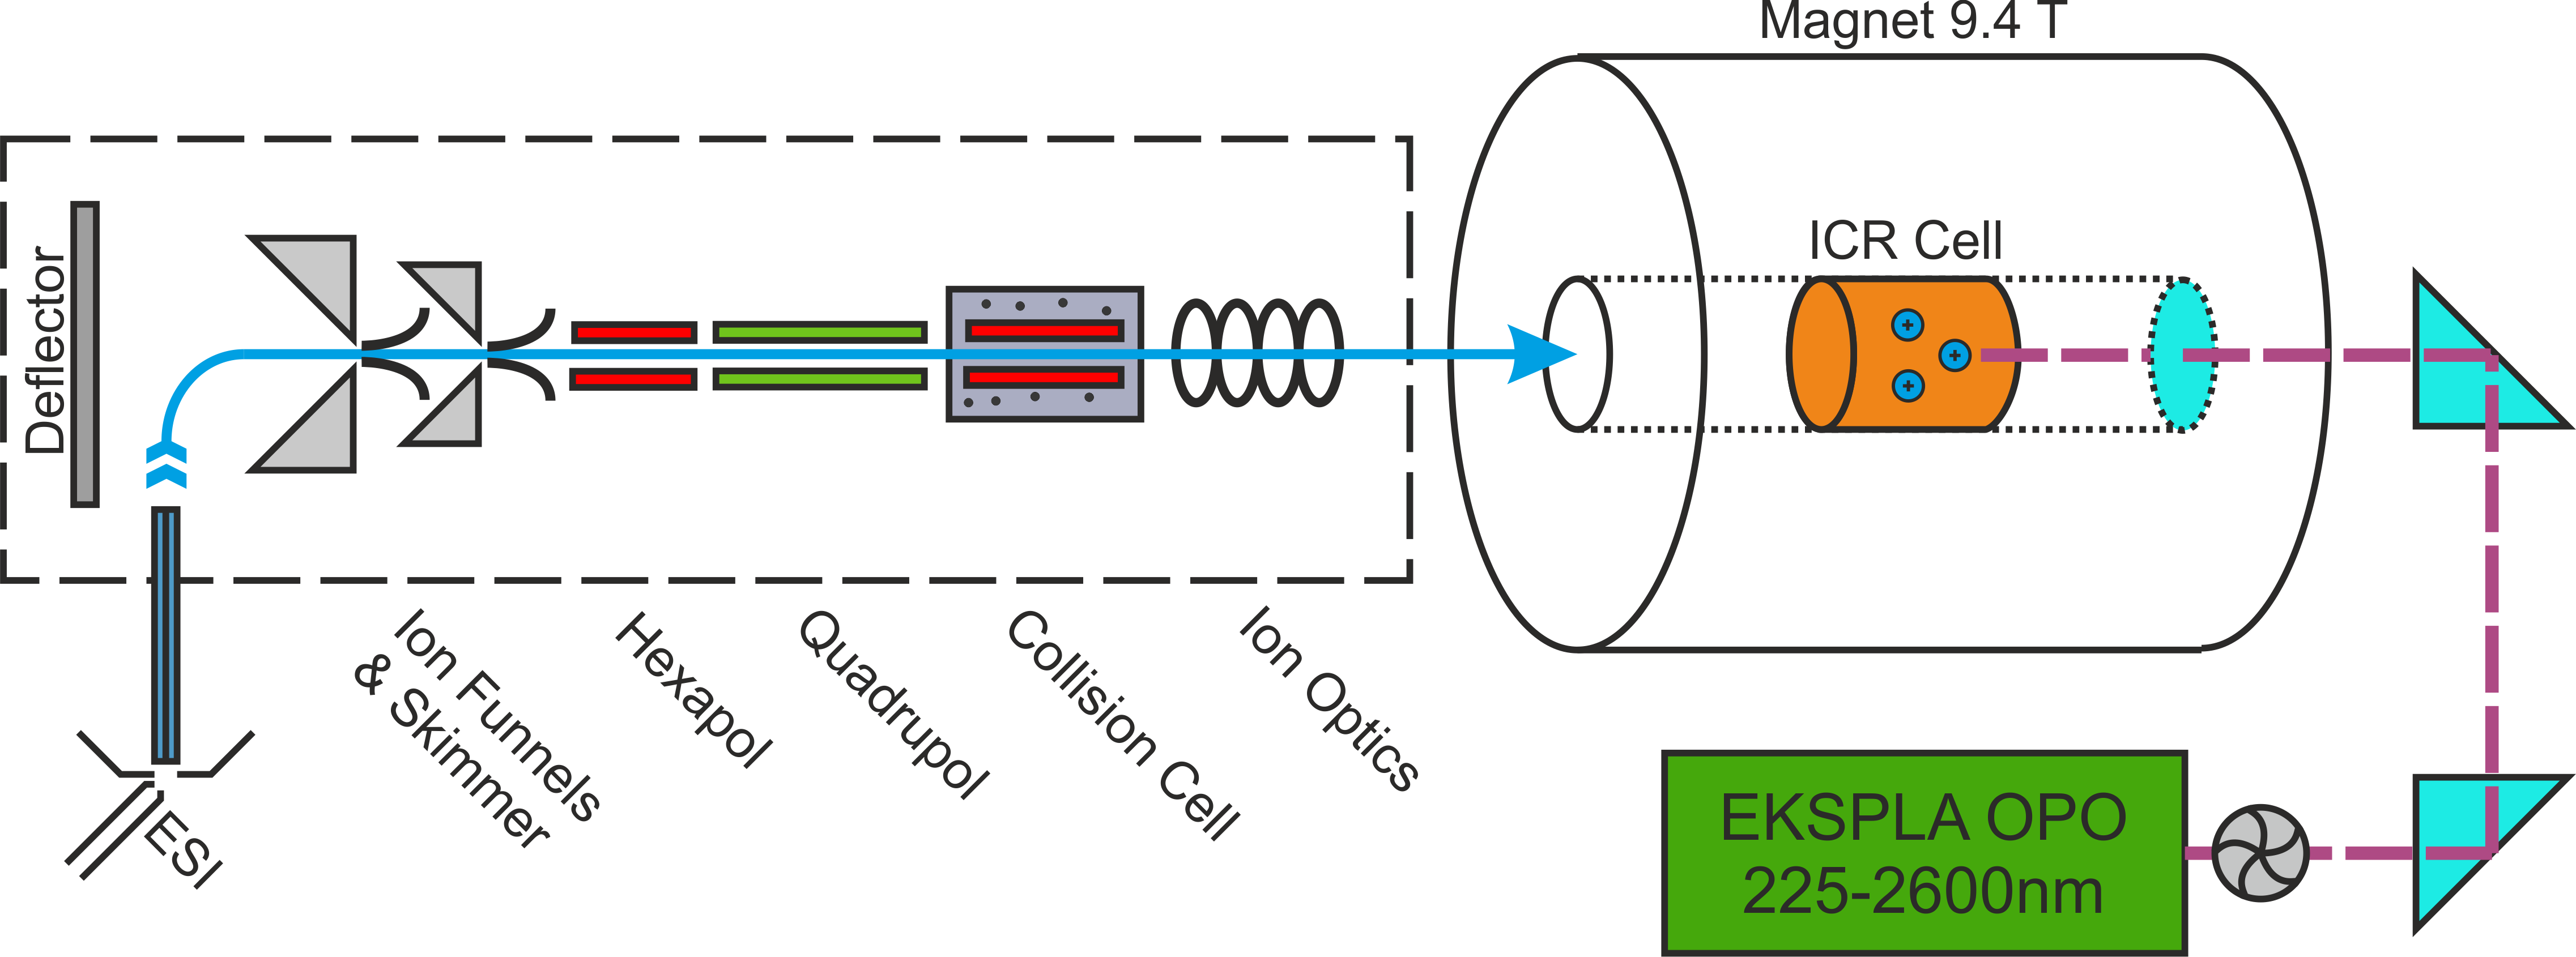
\includegraphics[width= 0.6 \textwidth]{setup.png}
	\caption{Sketch of the setup, taken from \cite{script}.}
	\label{fig_setup}
\end{figure}

\subsection{Ion Cyclotron Resonance Cell}
The ideas behind the ICR cell were already briefly laid out in Sec. \ref{sec_theory}, so here the focus is on the experimental implementation. \\
The cell used is of cylindrical shape and has to sets of electrodes to provide rotating electrical fields. Additionally, there are two more electrodes at the caps of the cylinder that generate an electric field along the direction of the magnetic field. This field has the purpose to keep the ions inside the cell, i.e. slow them down when they enter the cell, so the ion can be kept inside the ICR cell for a longer time. \\
The magnetic field in the cell is created with a superconducting \SI{9.4}{\tesla} magnet built around the ICR cell, as is shown in Fig. \ref{fig_setup}. 

%\subsection{Laser}

\section{Analysis}

\subsection{High resolution mass spectrum}
At the beginning of the experiment we had to record a high-resolution mass spectrum of Angiotensin with three additional protons attached to it (\ch{C62H92N17O14^{3+}}). In order to measure the spectrum we beforehand varied parameters in the setting, i.e. voltages for example on the ESI capillary, deflector, funnels etc, to maximize the intensity of the output. 
Then a spectrum was recorded over approximately \SI{40}{\minute}.\\
According to the Universal Mass Calculator \cite{umc}, this should yield an average $m/z$ ratio of \num{433.167}. This is only an average because in reality one would expect multiple peaks for different isotope combinations. As one can see in Fig. \ref{fig_hres_spectroscopy} there are in fact five peaks visible, although the last one is already hard to see. \\
Next, one can quickly estimate the resolution of the measured spectrum, so a Lorentzian curve was fitted to the highest peak in Fig. \ref{fig_hres_spectroscopy}, the fit can be seen in Fig. \ref{fig_fit_hires}. This yields a resolution of 
\begin{equation}
	\frac{m}{\Delta m_\mathrm{FWHM}} = \num{1.97(3) e6}.
\end{equation}
This value is now used to calculate the error of the peaks in Fig. \ref{fig_hres_spectroscopy}. The results we extracted from said figure were \SI{432.925013 \pm 0.00021945}{\atomicmassunit \per \elementarycharge} for the first peak, \SI{433.259529 \pm 0.00021962}{\atomicmassunit \per \elementarycharge} for the second one, and \SI{433.594038 \pm 0.00021979}{\atomicmassunit \per \elementarycharge}, \SI{433.928572 \pm 0.00021996}{\atomicmassunit \per \elementarycharge}, and \SI{434.263066 \pm 0.00022013}{\atomicmassunit \per \elementarycharge} respectively for the third, forth and fifth peak, as Tab. \ref{tab_peaks_spectrum} shows. 

\begin{figure}[htp!]
	\centering
	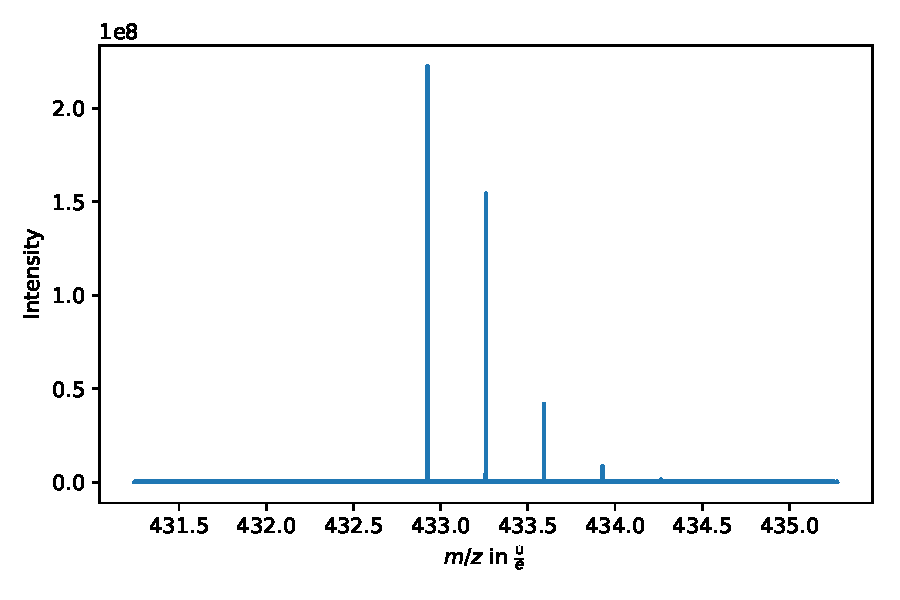
\includegraphics[width = 0.8 \textwidth]{hires_spectrum.pdf}
	\caption{Depiction of the measured data for the trice protonized Angiotensin. }
	\label{fig_hres_spectroscopy}
\end{figure}

\begin{table}
	\centering
	\caption{List of peak positions in Fig. \ref{fig_hres_spectroscopy}.}
	\begin{tabular}{c | c }
		Peak number & $m/z$ (\si{\atomicmassunit \per \elementarycharge})\\ \hline
		1 & \SI{432.925013 \pm 0.00021945}{ }\\
		2 & \SI{433.259529 \pm 0.00021962}{ }\\
		3 & \SI{433.594038 \pm 0.00021979}{ }\\
		4 & \SI{433.928572 \pm 0.00021996}{ }\\ 		
		5 & \SI{434.263066 \pm 0.00022013}{ }\\
	\end{tabular}
	\label{tab_peaks_spectrum}
\end{table}

\begin{figure}
	\centering
	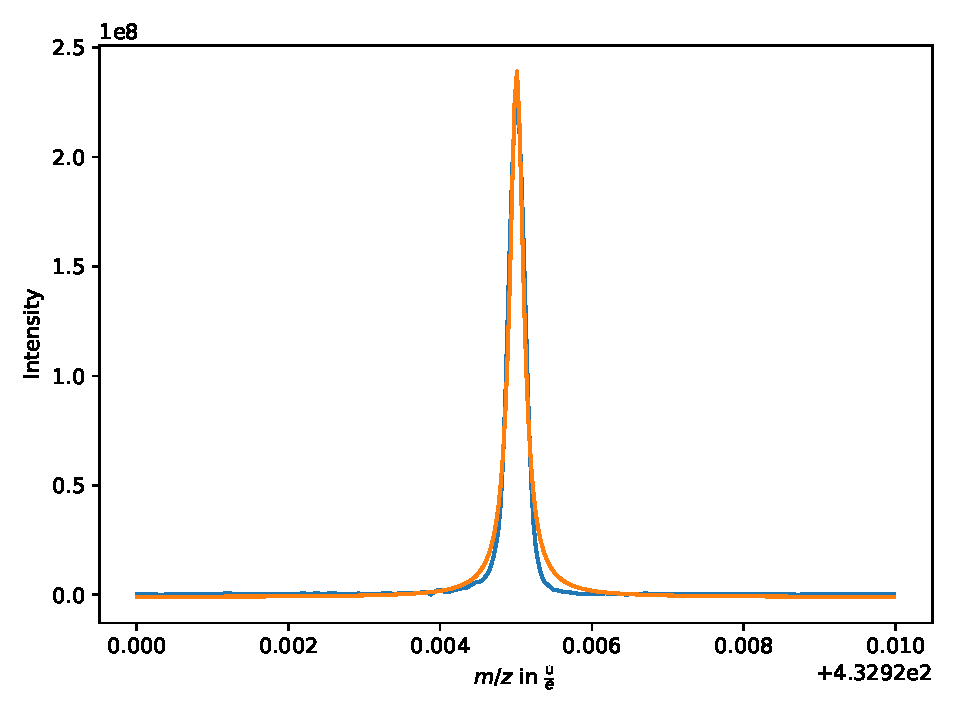
\includegraphics[width = 0.6 \textwidth]{fit_hires.pdf}
	\caption{Fitting a Lorentzian curve $y = A \frac{\gamma^2}{\gamma^2 + (x - x_0)^2} + b$ to the highest peak in the spectrum. The resulting parameters are $A = \num{2.40483457 \pm 0.0231878620 e8}$, $\gamma = \SI{1.09727221 \pm 0.0152696502 e-04}{\atomicmassunit \per \elementarycharge}$, $x_0 = \SI{432.925009(1)}{\atomicmassunit \per \elementarycharge}$, and $b = -\SI{1.07017512 \pm 0.228979314 e06}{}$. $A$ and $b$ are given in arbitrary units of intensity. }
	\label{fig_fit_hires}
\end{figure}

\subsection{CID fragment mass spectrum}

\subsection{SORI-CID fragment mass spectrum}

\begin{table}[htp!]
	\centering
	\caption{List of possible breaking points in peptide fragmentation notation of Roepstorff and Fohlman. The data was gathered with UMC \cite{umc}. }
	\begin{tabular}{c | c | c | c | c | c}
		Fragment & mass (${\mathrm{u}}/{e}$) & Fragment & mass (${\mathrm{u}}/{e}$) & Fragment & mass (${\mathrm{u}}/{e}$) \\ \hline
		$a_1$ & $88.085$ & $b_1$ & $116.095$ & $c_1$ & $131.11$ \\
		$a_2$ & $244.271$ & $b_2$ & $272.281$ & $c_2$ & $287.296$ \\
		$a_3$ & $343.402$ & $b_3$ & $371.412$ & $c_3$ & $286.427$ \\
		$a_4$ & $506.567$ & $b_4$ & $534.586$ & $c_4$ & $549.6$ \\
		$a_5$ & $619.733$ & $b_5$ & $647.744$ & $c_5$ & $662.758$ \\
		$a_6$ & $756.873$ & $b_6$ & $784.883$ & $c_6$ &  \\
		$a_7$ & $784.883$ & $b_7$ & $881.998$ & $c_7$ & $897.013$ \\
		$a_8$ & $1001.163$ & $b_8$ & $1029.173$ & $c_8$ & $1044.187$ \\
		$a_9$ & $1138.301$ & $b_9$ & $1166.312$ & $c_9$ & $1181.327$ \\
		$a_{10}$ & $1251.46$ & $b_{10}$ & $1279.47$ & $c_{10}$ &  \\
	\end{tabular}
	\label{tab_fragments}
\end{table}

\section{Conclusion}


\begin{thebibliography}{99}
\bibitem{electrospray}
\textsc{Simon J. Gaskell}, JOURNAL OF MASS SPECTROMETRY, VOL. 32, 677È688 (1997), \textit{Electrospray : Principles and Practice}, Michael Barber Centre for Mass Spectrometry, Department of Chemistry, UMIST, Manchester M60 1QD, UK

\bibitem{primer}
\textsc{Alan G. Marshall, Christopher L. Hendrickson, George S. Jackson}, \textit{FOURIER TRANSFORM ION CYCLOTRON RESONANCE MASS SPECTROMETRY: A PRIMER}, Center for Interdisciplinary Magnetic Resonance, National High Magnetic Field Laboratory, Florida State University, 1800 East Paul Dirac Dr., Tallahassee

\bibitem{script}
\textsc{Christian van der Linde}, \textit{Skriptum High Resolution Mass Spectrometry}, Universität Innsbruck

\bibitem{umc}
\textsc{Matthias Letzel}, \textit{Universal Mass Calculator - Student Edition}, Universität Münster, \url{https://www.uni-muenster.de/Chemie.oc/ms/downloads.html}
\end{thebibliography}

\end{document}
